% #############################################################################
% This is Chapter 4
% !TEX root = ../main.tex
% #############################################################################
% Change the Name of the Chapter i the following line
\fancychapter{Results}
\cleardoublepage
% The following line allows to ref this chapter
\label{chap:implement}

In this chapter, the results regarding the overall developed system for air quality monitoring and visualization with NB-IoT will be presented, as well as the performance of the considered SIMs. It will be divided into four sections, the PM10 Monitoring System experiment, SIMs performance, Online Data Visualization Web Application and finally Discussion. In this final section, the obtained results are addressed and analyzed in terms of what substantial inferences can be made regarding the experiments of this work.

For a better understanding of the results, it is important to note how PM10 concentrations affect air quality.
In \Cref{table:pm10-classification} one can see the official classification of the PM10 concentration values \cite{QualAr}.

\definecolor{springgreen}{rgb}{0.0, 0.65, 0.31}
\definecolor{carrotorange}{rgb}{0.93, 0.57, 0.13}
\definecolor{electricgreen}{rgb}{0.0, 1.0, 0.0}
\definecolor{bostonuniversityred}{rgb}{0.8, 0.0, 0.0}
\begin{table}[ht]
\centering
\caption{Classification of PM10 concentration values.}
\label{table:pm10-classification}
\begin{tabular}[t]{>{\centering}p{0.13\linewidth}>{\centering\arraybackslash}p{0.4\linewidth}}
\toprule
Classification&PM10 concentration interval (μg/m³)\\
\midrule
\cellcolor{electricgreen}Very Good& 0 - 20\\
\cellcolor{springgreen}Good& 21 - 35\\
\cellcolor{yellow}Medium& 36 - 50\\
\cellcolor{carrotorange}Weak& 51 - 100\\
\cellcolor{red}Bad& 101 - 1200\\
\bottomrule
\end{tabular}
\end{table}%

It can be observed that the smallest classification interval corresponds to a 14 μg/m³ variation, for both Good and Medium intervals. 
This value is useful to assess overall error results in relation to official metrics, for both the assessment of SIMs and the errors of measures between the developed system and reference monitors.


% #############################################################################
\section{NB-IoT PM10 Monitoring System}

This section objective is to describe the developed monitoring system performance and measures in comparison to the reference monitors, to later assess how it may integrate existing reference monitoring networks, which lack geographical density. Furthermore, the state and performance of the NB-IoT technology during the period of its use in this work is characterized.

\subsection{NB-IoT Coverage in Lisbon}

In \Cref{table:measurement-period} are presented the weeks during which the developed system was placed in a CCDR-LVT station. Colored cells represent the location where the developed sensor was placed during each week. In weeks colored in green, consistent measures were taken since there was NB-IoT coverage. On the other hand, in red colored weeks it was impossible to get consistent coverage and consequently no measures were obtained.

\definecolor{springgreen}{rgb}{0.0, 0.65, 0.31}
\definecolor{bostonuniversityred}{rgb}{0.8, 0.0, 0.0}
\renewcommand\arraystretch{1.5}
\renewcommand{\tabcolsep}{3pt}
\begin{table}[ht]
\centering
\caption{Weeks during which the developed system was placed next to a CCDR-LVT monitoring container.}
\label{table:measurement-period}
\begin{tabular}[t]{l>{\centering}p{0.06\linewidth}>{\centering}p{0.06\linewidth}>{\centering}p{0.06\linewidth}>{\centering}p{0.06\linewidth}>{\centering}p{0.06\linewidth}>{\centering}p{0.06\linewidth}>{\centering}p{0.06\linewidth}>{\centering}p{0.06\linewidth}>{\centering}p{0.06\linewidth}>{\centering\arraybackslash}p{0.06\linewidth}}
\toprule
&\multicolumn{2}{c}{July}&\multicolumn{4}{c}{August}&\multicolumn{4}{c}{September}\\
\midrule
{}Week&3&4&1&2&3&4&1&2&3&4\\
\midrule
AVL&\cellcolor{bostonuniversityred}&\cellcolor{bostonuniversityred}&&&&&&&\cellcolor{springgreen}&\cellcolor{springgreen}\\
ENC&&&\cellcolor{bostonuniversityred}&\cellcolor{bostonuniversityred}&\cellcolor{bostonuniversityred}&\cellcolor{bostonuniversityred}&\cellcolor{bostonuniversityred}&\cellcolor{bostonuniversityred}&&\\
\bottomrule
\end{tabular}
\end{table}

%%%%%%%%%%%%%%%%%%%%%%%%%%%%%%%%%%%%%%%%%%%%%%%%%%%%%%%%%%%%

\subsection{Evaluation of Obtained Measures}

From 13 to 26 September, measures obtained for each 15 minute interval were consistent and valid. The resulting data characteristics from these during this period are presented in \Cref{table:data-calibration-characteristics}.

\begin{table}[ht]
\centering
\caption{Data obtained during the measurement period.}
\label{table:data-calibration-characteristics}
\begin{tabular}[t]{>{\centering}p{0.13\linewidth}>{\centering}p{0.3\linewidth}>{\centering\arraybackslash}p{0.32\linewidth}}
\toprule
Full days&Obtained measures& Resulting hourly averages\\
\midrule
12&1195&298\\
\bottomrule
\end{tabular}
\end{table}%

Since data available from the reference monitor only corresponded to hourly averages, these were also calculated for the data obtained from the developed sensor, for comparison purposes. It is important to note that the reference monitor averages available online \cite{QualAr} are made for each hour with all the 15 minute spaced measures from the previous hour. Therefore, the same process was applied to calculate the developed system averages.

Statistics, such as the mean value, standard deviation and maximum and minimum values, regarding both obtained data sets were calculated and are presented in \Cref{table:error-measurement-period}.

\renewcommand\arraystretch{1.1}
\renewcommand{\tabcolsep}{1.4pt}
\begin{table}[ht]
\centering
\caption{Results of the measurement period, in (μg/m³).}
\label{table:error-measurement-period}
\begin{tabular}[t]{l>{\centering}p{0.15\linewidth}>{\centering}p{0.2\linewidth}>{\centering}p{0.2\linewidth}>{\centering\arraybackslash}p{0.2\linewidth}}
\toprule
{} &Mean value&Standard Deviation&Maximum value&Minimum value\\
\midrule
Reference Monitor&27.88&8.78&55.00&8.00\\
Developed System &15.04&10.64&56.80&2.49\\
\bottomrule
\end{tabular}
\end{table}

In \Cref{fig:system-calibration}, simultaneous measures of both sensors can be observed, for the whole time of placement of the developed system, along with the average RH values for the city of Lisbon.

\begin{figure}[ht]
\centering
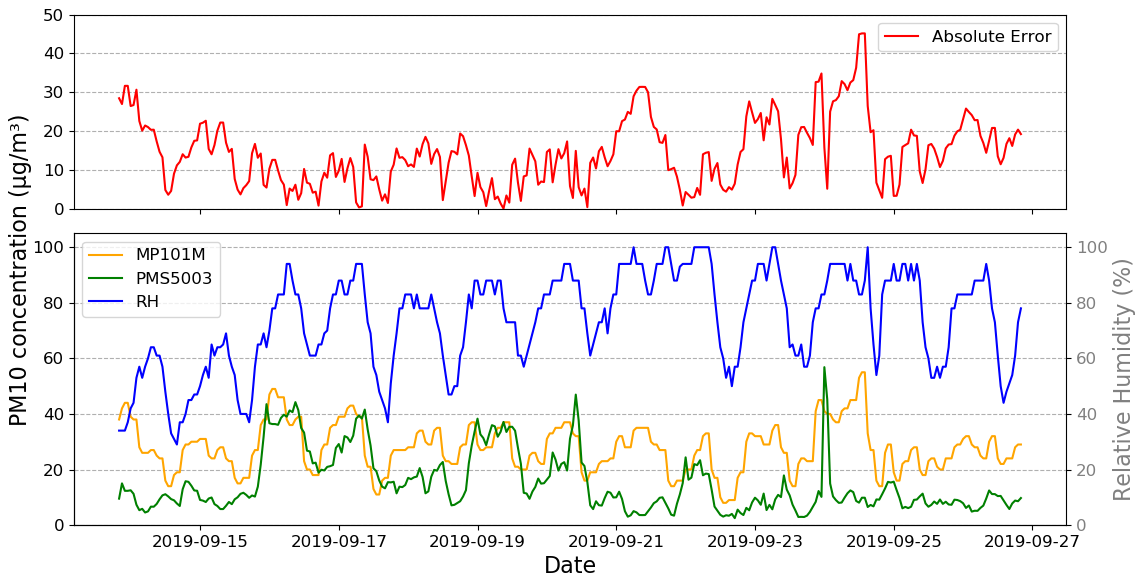
\includegraphics[width=1\textwidth]{./Images/Results/calibration2.png}
\caption{Time series of the PM10 concentrations reported by the sensors and corresponding RH.}
\label{fig:system-calibration}
\end{figure}

Several tendencies can be observed. The PMS5003 sensor often obtained lower measures. However, sometimes it peaked, surpassing the MP101M measures. This only happens for high values of RH. When the RH is decreasing, there is often less error between sensors.


The days 14, 15, 21 and 22 of September corresponded to weekend days, which means there is less car traffic in AVL. No meaningful tendencies were observed in these days, despite the average PM10 concentration being slightly lower in both sensors.

The average absolute error between the measures of the different sensors is 14.40 μg/m³. Furthermore, the scatter diagram in \Cref{fig:scatter-measurements} also highlights that the developed system measured values are predominantly lower than the reference measures.

\begin{figure}[ht]
\centering
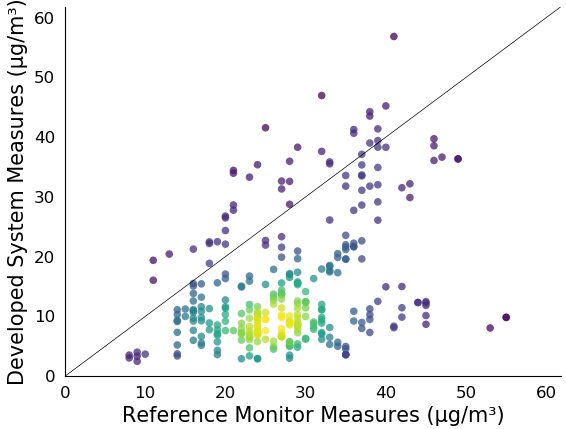
\includegraphics[width=0.55\textwidth]{./Images/Results/scatter-measurements.png}
\caption{Scatter diagram between the developed system and the reference monitor obtained measures.}
\label{fig:scatter-measurements}
\end{figure}

In the comparison of time series data, it is important to assess not only the error statistics between datasets, but also their linearity.
In order to identify correlations between different sensor readings, the Pearson coefficient was used. As explained in Section 3.2.1, the Pearson coefficient represents a measure of the linear correlation between two variables. The resulting coefficient varies from 1 to -1,  where 1 represents total positive linear correlation,  0 represents no linear correlation, and -1 total negative linear correlation.

The Pearson coefficient was calculated for every full day of the time series data, during the developed sensor placement. These and the overall Pearson coefficient are presented in \Cref{table:pearson-coefs-sensor}.

\renewcommand\arraystretch{1.5}
\renewcommand{\tabcolsep}{0.5pt}
\begin{table}[!htbp]
\centering
\caption{Pearson coefficients calculated for the full days of sensor positioning.}
\label{table:pearson-coefs-sensor}
\begin{tabular}[t]{>{\centering}p{0.07\linewidth}>{\centering}p{0.07\linewidth}>{\centering\arraybackslash}>{\centering}p{0.07\linewidth}>{\centering}p{0.07\linewidth}>{\centering}p{0.07\linewidth}>{\centering}p{0.07\linewidth}>{\centering}p{0.06\linewidth}>{\centering}p{0.07\linewidth}>{\centering}p{0.07\linewidth}>{\centering}p{0.07\linewidth}>{\centering}p{0.07\linewidth}>{\centering}>{\centering}p{0.07\linewidth}>{\centering\arraybackslash}p{0.1\linewidth}}
\toprule
\multicolumn{12}{c}{Day of placement (September of 2019)}&\multirow{2}{*}{Overall}\\\cline{1-12}
14&15&16&17&18&19&20&21&22&23&24&25&\\
\midrule
0.22&0.57&0.68&0.60&0.75&0.62&0.59&-0.23&0.57  &0.34&0.01&-0.37&0.39\\
\bottomrule
\end{tabular}
\end{table}%

The highest correlation coefficient corresponded to the fifth day of placement, 18 of September, in which the value of the coefficient was 0.75. The day with the lowest correlation values was the twelfth day, 25 of September, with a coefficient of -0.37. In terms of average errors, the day where higher absolute error was observed was 24 of September, with an error of 23.52 μg/m³, and the day with the lowest was 19 of September, with an error of 6.87 μg/m³. The measures corresponding to these days, as well as respective RH, are presented individually in \Cref{fig:worst-and-best}.

\begin{figure}[ht]
\centering
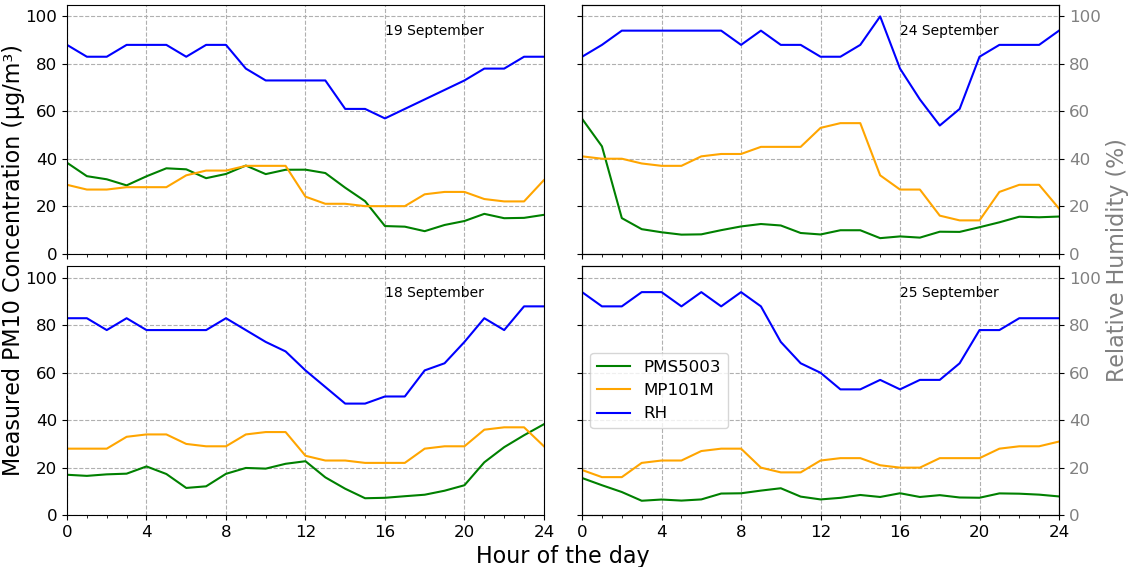
\includegraphics[width=1\textwidth]{./Images/Results/worst-and-best.png}
\caption{Measures of the days with the highest and lowest absolute errors and Pearson coefficients.}
\label{fig:worst-and-best}
\end{figure}

\pagebreak
%
% #############################################################################
\section{SIMs Testing}

In this section, SIM parametrization and performance results are presented. In the parametrization phase, the main objective is to define the best parameters for every interpolation algorithm, with main focus on FBN, which is the less documented algorithm. In both phases, error statistics are calculated in order to define whether there is an algorithm which performance stands out from the remaining.

%%%%%%%%%%%%%%%%%%%%%%%%%%%%%%%%%%%%%%%%%%%%%%%%%%%%%%%%%%%%%%%%%%%%%%%%
%               Parametrization Results
%%%%%%%%%%%%%%%%%%%%%%%%%%%%%%%%%%%%%%%%%%%%%%%%%%%%%%%%%%%%%%%%%%%%%%%%
\subsection{SIM Parametrization}

The used algorithms which have user defined parameters are IDW, OK and FBNs. In this section these parameters are tested in what regards error statistics in the 5 year dataset.

In IDW, the only user defined parameter is the power function. Through the cross validation approach application in the dataset, the power function with the best error statistics was chosen. Values of \textit{p} from 0 to 5 were tested. Results are presented in \Cref{table:idw-params}, and the value selected, which has the lowest overall MAE and RMSE values is \textit{p} = 0. 

\renewcommand\arraystretch{1.5}
\begin{table}[ht]
\centering
\caption{IDW power function comparison results.}
\label{table:idw-params}
\begin{tabular}[t]{>{\raggedright}p{0.05\linewidth}>{\centering}p{0.11\linewidth}>{\centering}p{0.11\linewidth}>{\centering}p{0.11\linewidth}>{\centering}p{0.11\linewidth}>{\centering}p{0.11\linewidth}>{\centering}p{0.11\linewidth}>{\centering}p{0.11\linewidth}>{\centering\arraybackslash}p{0.11\linewidth}}
\toprule
\multirow{2}{*}{\textit{p}}&\multicolumn{2}{c}{ENC}&\multicolumn{2}{c}{ODI}&\multicolumn{2}{c}{REB}&\multicolumn{2}{c}{SCB}\\
\cline{2-9}
&MAE&RMSE&MAE&RMSE&MAE&RMSE&MAE&RMSE\\
\midrule
0&4.57&6.34&4.97&6.59&5.79&7.37&11.15&14.88\\
1&4.74&6.25&4.97&6.62&7.19&9.04&10.73&14.34\\
2&5.69&7.38&5.15&6.88&9.40&11.94&11.06&14.64\\
3&6.80&8.79&5.61&7.52&11.11&14.33&11.80&15.42\\
4&7.76&10.06&6.17&8.26&11.92&15.49&12.47&16.15\\
5&8.54&11.09&6.60&8.86&12.24&15.94&12.90&16.62\\
\bottomrule
\end{tabular}
\end{table}

The same approach was applied in the parameter assessment of the remaining algorithms.

In OK, the variogram is the main user defined parameter. As stated in Section 3.2.2, the dataset used in this work's problem has a very low number of data points, which are sparsely located in space. This problem makes it not viable to define a custom variogram for the OK interpolation. Therefore, several pre-defined variograms were tested, in order to identify which was the most suitable for this specific interpolation problem. 

The obtained results are presented in \Cref{table:kriging-params}. The variogram model which has the lowest overall MAE and RMSE values is the linear model. 

\renewcommand\arraystretch{1.5}
\begin{table}[ht]
\centering
\caption{OK variogram comparison results.}
\label{table:kriging-params}
\begin{tabular}[t]{>{\raggedright}p{0.12\linewidth}>{\centering}p{0.1\linewidth}>{\centering}p{0.1\linewidth}>{\centering}p{0.1\linewidth}>{\centering}p{0.1\linewidth}>{\centering}p{0.1\linewidth}>{\centering}p{0.1\linewidth}>{\centering}p{0.1\linewidth}>{\centering\arraybackslash}p{0.1\linewidth}}
\toprule
\multirow{2}{*}{Variogram}&\multicolumn{2}{c}{ENC}&\multicolumn{2}{c}{ODI}&\multicolumn{2}{c}{REB}&\multicolumn{2}{c}{SCB}\\
\cline{2-9}
&MAE&RMSE&MAE&RMSE&MAE&RMSE&MAE&RMSE\\
\midrule
Linear&4.95&6.68&5.03&6.69&5.88&7.52&10.89&14.51\\
Gaussian&5.96&8.02&5.38&7.29&8.93&12.23&11.21&14.69\\
Exponential&5.42&7.24&5.14&6.87&7.28&9.38&10.94&14.49\\
Spherical&5.72&7.66&5.25&7.04&8.24&10.77&11.19&14.69\\
Power&4.97&6.68&5.08&6.77&6.12&7.89&10.88&14.49\\
Hole-effect&4.77&6.62&5.03&6.65&5.95&7.57&11.36&15.08\\
\bottomrule
\end{tabular}
\end{table}

In what regards FBN interpolation, an higher number of parameters need to be addressed, namely both testing and training epochs, the network size, the number of samples made by each neuron and the granularity of the memories of each consequent neuron.

Tests were made with several samples, with 2000 iterations, from the dataset, with the objective to assess the set of training and testing epochs, and the set of the net size, number of samples and granularity, independently, as can be observed in \Cref{table:fbn-parametrization}.

\renewcommand\arraystretch{1.5}
\begin{table}[ht]
\centering
\caption{FBN Parametrization assessment results.}
\label{table:fbn-parametrization}
\begin{tabular}[t]{>{\centering}p{0.1\linewidth}>{\centering}p{0.1\linewidth}>{\centering}p{0.1\linewidth}>{\centering}p{0.1\linewidth}>{\centering}p{0.1\linewidth}>{\centering}p{0.175\linewidth}>{\centering\arraybackslash}p{0.175\linewidth}}
\toprule
Training Epochs&Testing Epochs&Net Size&Samples&Granularity&RMSE (μg/m³)&MAE (μg/m³)\\
\midrule
%TODO:
10&10&15&4&2&13.99&18.35\\
50&50&15&4&2&13.63&17.96\\
\midrule
%TODO:
10&10&75&9&3&11.22&14.80\\
50&50&75&9&3&10.98&14.54\\
\midrule
%TODO:
10&10&125&16&4&12.94&16.91\\
50&50&125&16&4&12.05&15.92\\
\bottomrule
\end{tabular}
\end{table}

From further studying and experimenting with FBNs, it was observed that:

\begin{itemize}
    \item Performance increased with the number of testing and training epochs;
    \item Similarly to the observed in other studies \cite{Tome2014}, the number of samples should be substantially lower than the net size;
    \item When very low granularity values are used, consequent neurons will have very small memory tables. Therefore, the information sampled in sampling phases, in both learning and testing epochs, will have insufficient resolution;
    \item For high granularity values, the number of testing and learning epochs needs to be higher, than with values close to the square root of number of samples.
    \item As also pointed in previous studies, FBNs advantages lie in their ability to obtain very good results without extensive parameterization efforts \cite{Tome2014}.
\end{itemize}

% Discussion - FBNs
%The following statements can be concluded from these %results:
%\begin{itemize}
%    \item Testing and training epochs do not have %influence in the results;
%    \item Net size, along with the number of samples %and granularity increase leads to consistently %better results, in terms of both \ac{MAE} and %\ac{RMSE}.
%\end{itemize}

% Discussion - FBNs
% A substantial increase in computing times with the increase of the network size was observed. If larger network sizes would be used, with large datasets, execution times would increase to impractical values.

The chosen parameters for the FBN interpolation, accounting the previous results, are presented in \Cref{table:fbn-chosen-parameters}.

\renewcommand\arraystretch{1.5}
\begin{table}[ht]
\centering
\caption{Choice of parameters for FBNs used in this work.}
\label{table:fbn-chosen-parameters}
\begin{tabular}[t]{>{\centering}p{0.17\linewidth}>{\centering}p{0.17\linewidth}>{\centering}p{0.17\linewidth}>{\centering}p{0.17\linewidth}>{\centering\arraybackslash}p{0.17\linewidth}}
\toprule
Training Epochs&Testing Epochs&Net Size&Samples&Granularity\\
\midrule
50&50&75&9&3\\
\bottomrule
\end{tabular}
\end{table}

FBN interpolation performance was also tested using the dataset with measures corresponding to 15 minute intervals, as referred in Section 3.2.3. This test main objective is to analyze how resolution of data influences FBNs interpolation performance.

The resulting error statistics are presented in \Cref{table:fbn-15mins}.

\renewcommand\arraystretch{1.5}
\begin{table}[ht]
\centering
\caption{FBN 15 minute improvements.}
\label{table:fbn-15mins}
\begin{tabular}[t]{l>{\centering}p{0.08\linewidth}>{\centering}p{0.08\linewidth}>{\centering}p{0.08\linewidth}>{\centering}p{0.08\linewidth}>{\centering}p{0.08\linewidth}>{\centering}p{0.08\linewidth}>{\centering}p{0.08\linewidth}>{\centering}p{0.08\linewidth}>{\centering}p{0.08\linewidth}>{\centering\arraybackslash}p{0.08\linewidth}}
\toprule
&\multicolumn{2}{c}{AVL}&\multicolumn{2}{c}{ENC}&\multicolumn{2}{c}{OLI}&\multicolumn{2}{c}{RES}&\multicolumn{2}{c}{SCB}\\
\midrule
{} &MAE&RMSE&MAE&RMSE&MAE&RMSE&MAE&RMSE&MAE&RMSE\\
\midrule
Regular FBN      & 8.36 & 10.99 & 7.18 & 9.52  & 9.72  & 11.97 & 6.05 & 9.38  & 6.53 & 9.68\\
15min FBN        & 9.42 & 12.49 & 8.87 & 11.87 & 10.77 & 13.35 & 6.72 & 10.41 & 6.50 & 10.17\\

\bottomrule
\end{tabular}
\end{table}

% TODO: alterar estes valores quando atualizar a tabela
In the regular FBN execution these values were 7.57 and 10.57, which are better than the 15 minute implementation, which were 8.46 and 11.71. 


% Discussion - FBNs
%Worse performance was observed in the FBN execution with the 15 minute interval resolution, which leads to the conclusion that the number of training rules used for each interpolation has no influence on the overall inference performance of FBNs.

%
%%%%%%%%%%%%%%%%%%%%%%%%%%%%%%%%%%%%%%%%%%%%%%%%%%%%%%%%%%%%%%%%%%%%%%%%
%               SIM comparison results and analysis
%%%%%%%%%%%%%%%%%%%%%%%%%%%%%%%%%%%%%%%%%%%%%%%%%%%%%%%%%%%%%%%%%%%%%%%%

\subsection{SIM Comparison}

Every algorithm considered so far in this work was tested with the cross validation approach in the 5 year dataset. 
%Other simpler interpolation algorithms, with no user defined parameters, were additionally added to the tests, namely the Linear Interpolation and the Nearest Neighbors interpolation algorithms.

Results regarding the error statistical parameters MAE and RMSE of every algorithm are presented in table \Cref{table:sim-comparison}, for a total of 43 956 single inferences each.

\renewcommand\arraystretch{1.5}
\begin{table}[ht]
\centering
\caption{Model comparison results.}
\label{table:sim-comparison}
\begin{tabular}[t]{l>{\centering}p{0.1\linewidth}>{\centering}p{0.1\linewidth}>{\centering}p{0.1\linewidth}>{\centering}p{0.1\linewidth}>{\centering}p{0.1\linewidth}>{\centering}p{0.1\linewidth}>{\centering}p{0.1\linewidth}>{\centering\arraybackslash}p{0.1\linewidth}}
\toprule
&\multicolumn{2}{c}{ENC}&\multicolumn{2}{c}{ODI}&\multicolumn{2}{c}{REB}&\multicolumn{2}{c}{SCB}\\
\midrule
{} &MAE&RMSE&MAE&RMSE&MAE&RMSE&MAE&RMSE\\
\midrule
IDW&4.65&6.52&4.89&6.48&5.46&6.97&11.52&15.31\\
OK&4.67&6.52&4.89&6.49&5.55&7.06&11.41&15.18\\
FBN&5.82&7.62&6.36&8.41&7.55&9.62&11.08&14.75\\
Linear&5.90&7.74&6.59&9.46&10.11&13.11&11.04&14.51\\
NearestN&11.20&14.63&7.35&9.82&12.58&16.36&13.45&17.22\\
\bottomrule
\end{tabular}
\end{table}


The algorithms with the overall lower MAE and RMSE results were IDW, with 6.42 μg/m³ and 9.25 μg/m³, respectively, and OK, with 6.42 μg/m³ and 9.23 μg/m³. NN with 11.03 μg/m³ and 14.66 μg/m³, had the worse results, followed by LI, with 8.28 μg/m³ and 11.36 μg/m³. FBN results were 7.55 μg/m³ and 10.24 μg/m³. Density scatter diagrams and histograms of the IDW, OK and FBN algorithms can be observed in \Cref{fig:performance-scatter-diagrams} and \Cref{fig:performance-histograms}. % TODO


% TODO Mudar para os anexos.
\begin{figure}[ht]
\centering
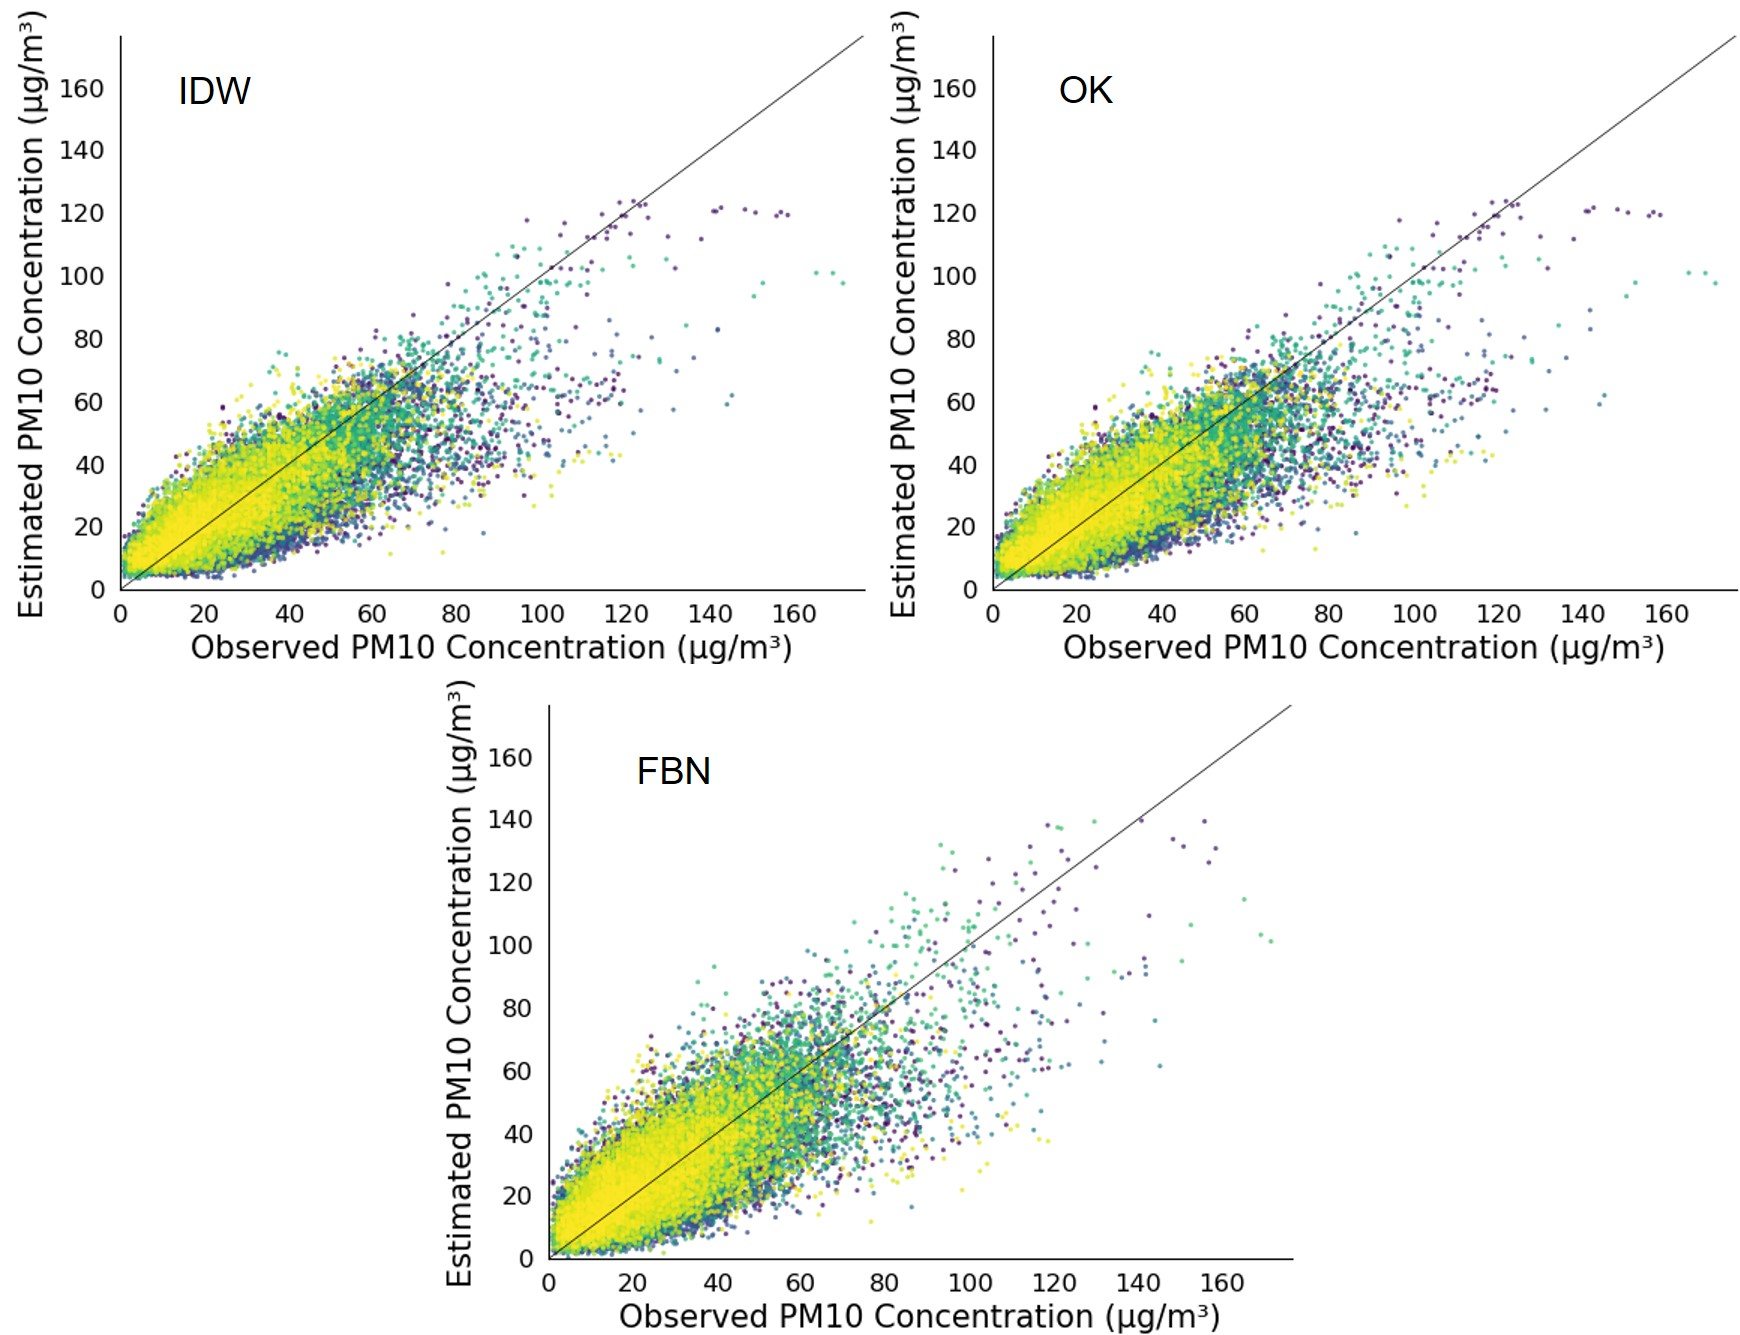
\includegraphics[width=0.8\textwidth]{./Images/Results/performance-scatter-diagrams.jpg}
\caption{Scatter diagrams obtained from 43 956 inferences for IDW, OK and FBN, respectively.}
\label{fig:performance-scatter-diagrams}
\end{figure}

It should additionally be noted that FBNs execution times of the obtained results took approximately 9 hours, while every remaining algorithm only took from 5 to 10 minutes interpolating through the entire dataset.

% Discussion - FBNs
%This again adds to the conclusion that FBNs have less practical application in large dataset problems.

% Discussion - Algorithms
%It is important to note that despite worse values RMSE and MAE for the FBNs, these still represent error values which are under variations of 14 μg/m³, which corresponds to the smallest classification interval of the \ac{PM10} concentration values official classification.

\begin{figure}[ht]
\centering
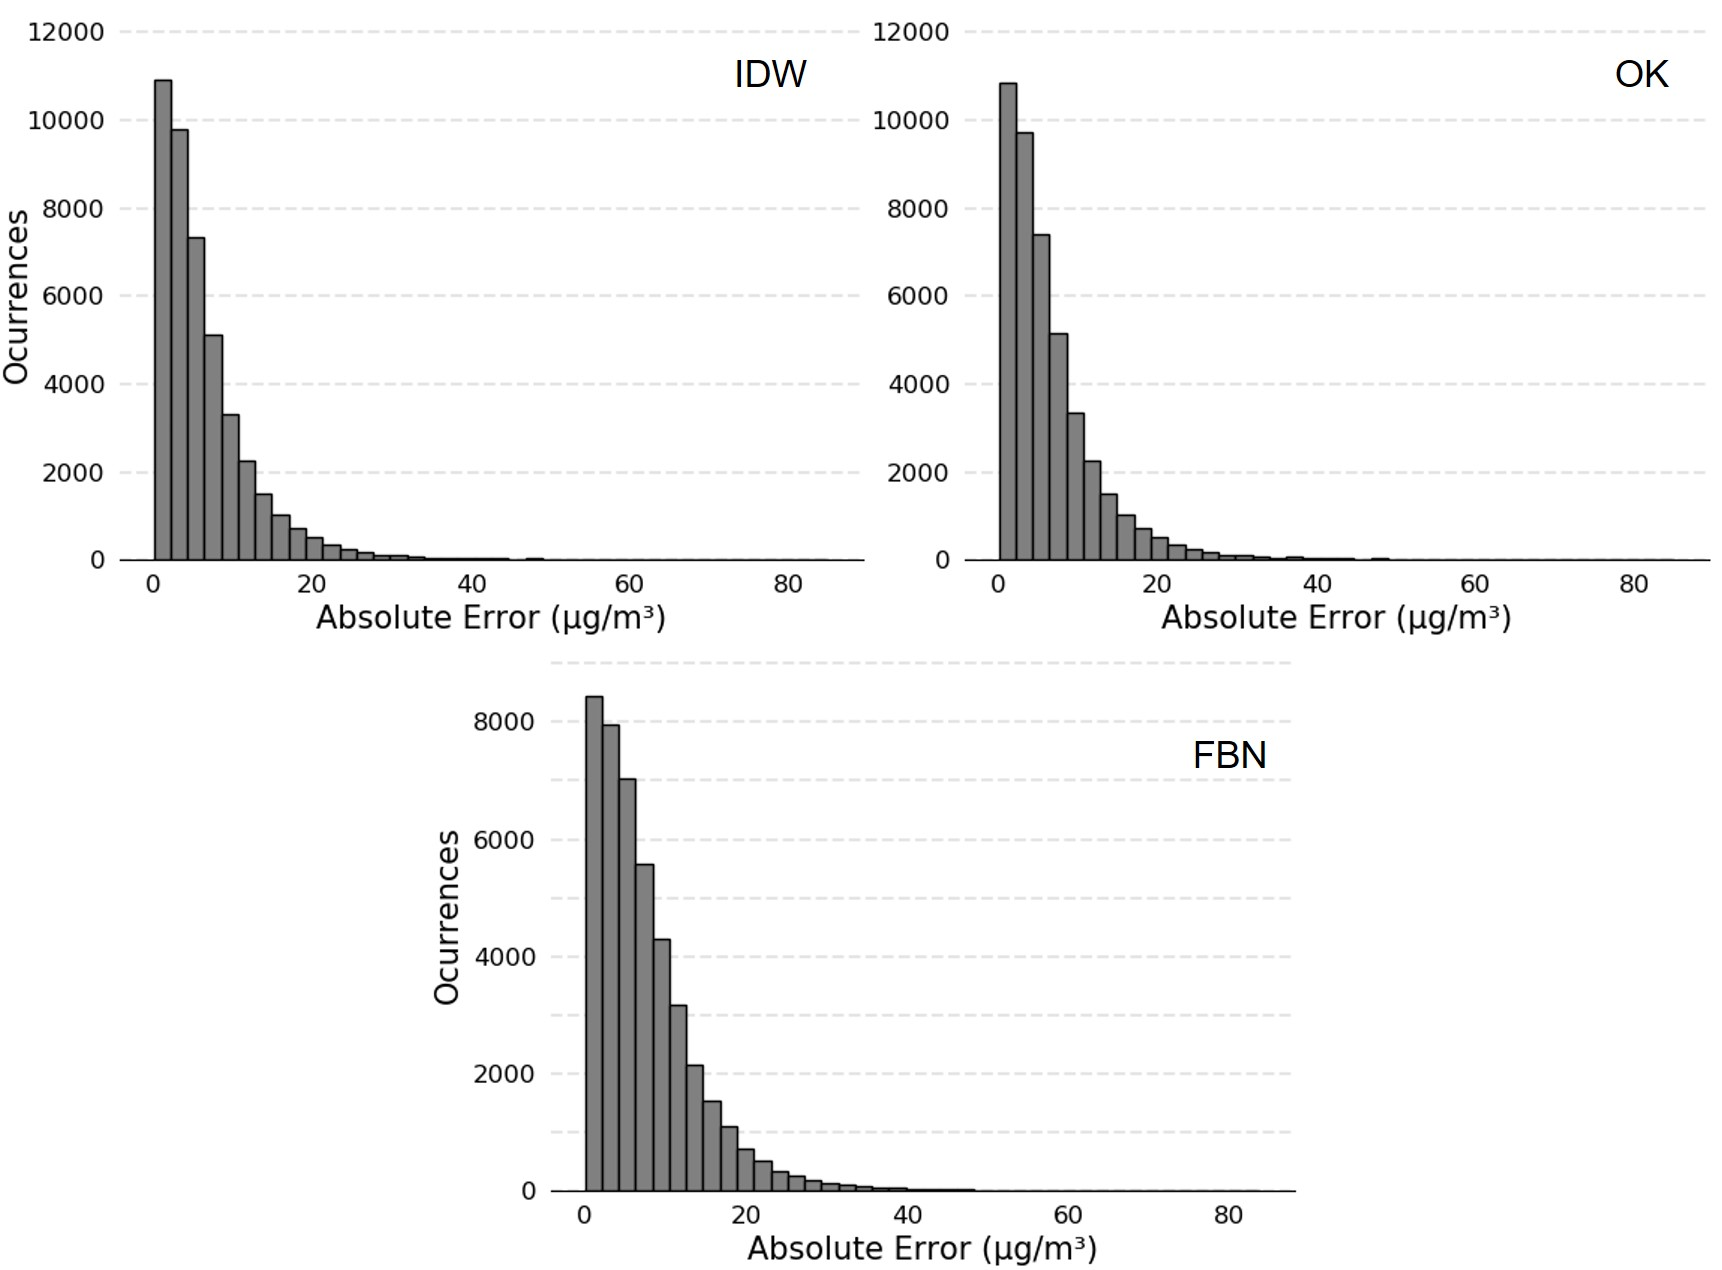
\includegraphics[width=0.8\textwidth]{./Images/Results/performance-histograms.jpg}
\caption{Histograms obtained from 43 956 inferences for IDW, OK and FBN, respectively.}
\label{fig:performance-histograms}
\end{figure}

% Para introduzir aqui secção sobre as FBNS:
%- mencionar em: 
%   - introducao capitulo 4, discussao, e conclusao.

%
% É concluído que nao ha correlação espacial suficiente para que sejam retiradas conclusoes relativamente ao desempenho das FBNs em interpolação espacial.
% Esta secção terá uma ou duas experiencias com dados estocasticos simulados e de alta correlação espacial, num plano, para fazer inteprolação 2d com as fbns e testar a sua performance contra outros algoritmos num ds com alta spatial autocorrelation.

\section{Online Data Visualization Web Application}

The developed PM10 visualization application was created to present a tool to visualize tested geographical interpolation algorithms and also to constitute a prototype for a platform of live online visualization of interpolated air quality related phenomena.

The resulting prototype is an application with PM10 interpolated data for the city of Lisbon. It has a resolution of 100 meters, both in color and in height of the pollution surface. It provides the possibility to hover over to know estimated PM10 concentration values in any location inside the outline defined by the CCDR-LVT monitoring network stations.

The application design is focused in the user experience, and allows the user to zoom in and out, and change both pitch and bearing of the map.

The final result of the developed web application is presented in \Cref{fig:developed-visualization} and is available at \url{http://138.68.165.208/}.

% Alterar esta figura para uma mais atualizada
\begin{figure}[ht]
\centering
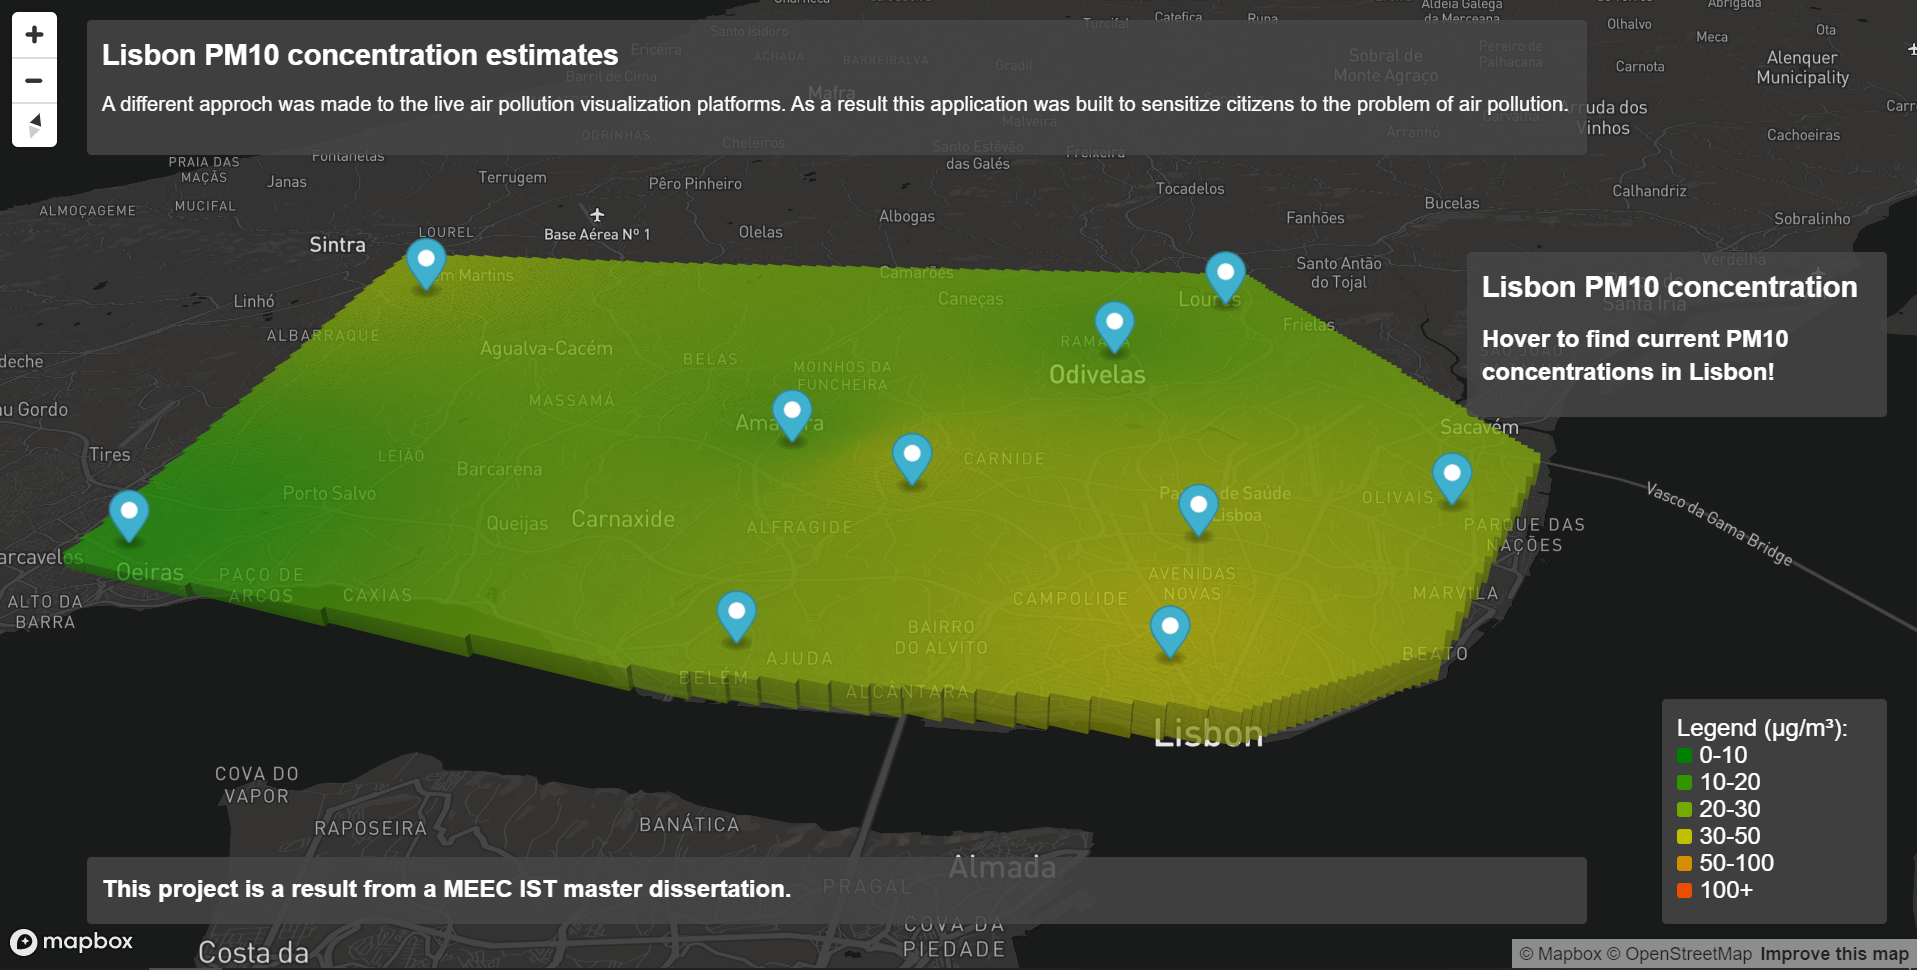
\includegraphics[width=1\textwidth]{./Images/Results/developed-visualization.PNG}
\caption{Developed web application final result, with live data from QualAr, interpolated with OK.}
\label{fig:developed-visualization}
\end{figure}

In \Cref{table:access-times} are presented the access times of some of the platforms for air pollution visualization referenced in this work, on comparison to the developed one. These results were provided from tests from Pingdom tool for web page performance assessment \cite{pingdom}.

\begin{table}[ht]
\centering
\caption{Access times of various air quality visualization web pages.}
\label{table:access-times}
\begin{tabular}[t]{l>{\centering}p{0.18\linewidth}>{\centering}p{0.13\linewidth}>{\centering\arraybackslash}p{0.16\linewidth}}
\toprule
Web Page&Access Time (ms)&Requests&Page Size (MB)\\
\midrule
138.68.165.208 (developed application)&207&44&7.5\\
airindex.eea.europa.eu&2580&77&3.8\\
qualar.apambiente.pt&3400&180&9.1\\
breezometer.com/air-quality-map/city/lisbon&3629&184&2.2\\
\bottomrule
\end{tabular}
\end{table}

% Se houver tempo, optimizar o ficheiro geojson https://docs.mapbox.com/help/troubleshooting/working-with-large-geojson-data/
% e colocar aqui uma tabela com tempos de acesso a alguns websites



\section{Discussion}

Results obtained and presented in this chapter are discussed in this section.

\subsection{Developed PM10 Monitoring System}

%%
Regarding the NB-IoT coverage in Portugal, from both MEO and NOS, namely in the capital Lisbon, it could be concluded that it is not good enough for professional applications at the time of this work.
During the 10 weeks of placement of the developed system, in different locations in the city of Lisbon, there were only 2 weeks when it was possible to get consistent coverage.

According to its specifications, overviewed in Section 2.4.4, NB-IoT has one of the widest coverages between IoT technologies. This was not observed in this work. It might have happened because NB-IoT is still in early implementation stages in Portugal.

These results demonstrate that the developed sensor, at the time of this work, from the network coverage perspective, can not be employed neither integrate current official monitoring networks.

Before assessing the used low-cost sensor performance, it is important to note that the obtained data only corresponds to a period of approximately two weeks as presented in \Cref{table:measurement-period}, which represents a small sample size in comparison to what was expected, due to the NB-IoT network coverage constraints.


% observations

During the sensor placement and comparison period, the PMS5003 sensor often obtained lower measures. However, sometimes it peaked, surpassing the MP101M measures. This only happened for high values of RH. It additionally can be observed in \Cref{fig:system-calibration} that when the RH is decreasing is when often less error is observed between the sensors.

% error statistics
The average absolute error between the measures of the different sensors (14.40 μg/m³) is slightly above the smallest scale division in \Cref{table:pm10-classification}. In the scatter diagram of \Cref{fig:scatter-measurements} it can be observed that the developed system measured values are predominantly lower than the reference measures. The daily pearson correlation coefficients (\Cref{table:pearson-coefs-sensor}) showed inconsistency in the linearity between sensor readings.

%temperature
PMS5003 sensor manufacturers claim that the sensor presents high consistency in the temperatures between 10 and 40ºC \cite{Sayahi2018}. It was summer season during this experiment, and the temperature values never exceeded positively nor negatively the above mentioned interval. 
However, the reference monitor has a controlled sampling flow rate of 1 m³/h, as well as a temperature-regulated sampling tube. This does not happen in the PMS5003, in which neither air flow nor its temperature are controlled.
Furthermore, it is important to note that the low-cost sensor was placed in the outside of the monitoring container, while the reference monitor was placed on the inside.

% rain
The only rain occurrences during the placement periods happened in the day 21 of September. It is the day with the second highest absolute error between readings, and PMS5003 measures were very low in comparison to the MP101M.

% humidity
In a study by Zheng et al., in 2018, a similar sensor model (PMS3003) was extensively tested against professional reference monitors and it was observed that while temperature took a negligible part in the difference observed between sensors, RH had a considerable influence in the deviation observed in the low-cost sensor \cite{Zheng2018}. This can be the one cause for the high observed error and linearity inconsistencies in this work experiment.

Humidity can have a negative effect on electronic circuits, such as the one in the developed system. However, no recurrent effects were observed due to humidity peaks specifically in the PMS5003 readings.

The registered high humidity intervals correspond to night and dawn periods. Similar to what happened in a study by Jayaratne et al., in 2018, in these periods, measures are often higher than in the rest of the time. The increase of measured values when there is high humidity is expected in the PMS5003 due to its documented humidity sensitivity, however it suggests that the MP101M is also influenced by high RH.

In the same study, it was stated that above 75\% humidity, marked effects are seen in low-cost sensors due to air particle size growth by deliquescence, specially if these do not have drying facilities at the sample inlets \cite{Jayaratne2018}. However, in this work, no effect in the PMS5003 was observed in high humidity periods. There is a substantial increase in measured values, but coincident with the increase reported by the MP101M, and there are undervalued measurements during the rain periods.

% car traffic
The days 14, 15, 21 and 22 of September corresponded to weekend days, which often means there is less car traffic in AVL. No meaningful tendencies were observed in these days, despite the average PM10 concentration being slightly lower in both sensors.

During the day, MP101M readings are mostly higher than PMS5003's.
According to Jayaratne et al., in the same study \cite{Jayaratne2018}, this may happen because the size of traffic particles are below the minimum detectable size limit of low-cost sensors, which for the PMS5003 is 0.3 µm (300 nm). As presented in a study by Li et al., in 2018, where the size-resolved mass concentration of volatile and non-volatile components of vehicle emitted particles is studied, the diameter of particles emitted by vehicles was mostly below 300 nm, which corroborates the fact these are not accordingly measured by the PMS5003 \cite{Li2018}.

% conclusion on placement in official networks
The objective of this experiment was to find out whether it is possible to define a correction factor for the low-cost sensors, through which they could provide PM10 readings with very low error in comparison with reference monitors. Results show that the absolute error between sensors is not linear neither correlated with the absolute value of RH. Therefore appropriate correction factors are not possible to derive with the obtained data.

Due to the numerous disadvantages observed in this work, it can be concluded, with this work data, that low-cost sensors are not suited for regulatory applications, such as assess if the air quality meets stipulated guidelines for particle pollution. However, with previous study of the placement location, such as average particle size and overall RH, and the deduction of a fitting correction factor to that specific location, it could be used for informative purposes, for example in interpolation platforms, to provide a better resolution to monitoring networks which currently suffer from sparsity.

% Comparing conclusions to other works conclusions
In mentioned studies concerning PMS low-cost sensor calibration, it was concluded that appropriate calibration models using dynamic adjustments for meteorological parameters are an essential prerequisite for these sensors to achieve high accuracy and precision in the ambient monitoring and that after proper calibration, low-cost PM sensors can be promising monitors for PM sensor network development and to complement the existing networks, without specifying its integration in official networks \cite{Zheng2018}.


%One calibration approach which could be considered, through what is observed in \Cref{fig:scatter-measurements}, which are predominantly lower measured values in the low-cost sensor, is the simple increase of the values below 10 ug/m3 to the double of its value, which would reduce the error between measures. This could lower the error only to a certain value, however it is not considered to be good enough as a calibration function, since it only covers a small number of measures, and the special case of low pollution. It also would not allow the sensor to take accurate enough measures for it to be used as a data point for interpolations and even in terms of integration in the official monitoring networks.


\subsection{SIMs Assessment}

The algorithms with the best overall performance were IDW and OK, followed by FBNs, LI and lastly NN.

In \Cref{table:correlation-coef}, correlation coefficients between every station of the dataset was calculated. It can be observed that the stations with the highest correlation coefficients between them were relatively close in terms of geographical location, despite an overall big correlation observed between almost every station.

The high performance of IDW with \textit{p} = 0, which means that distance between data points is not considered for the calculation of the interpolated values, suggests that the distance correlation between stations is low.

%This could help formulate the hypotheses of the high spatial correlation between stations. However, the fact that an algorithm where distances between station was the one with the best performance leads to the conclusion that this hypotheses is not valid.

Air dispersion and movement in urban environments is an environmental problem of high complexity, due to its influence by many factors. In the last 5 years, in the city of Lisbon, the dataset reveals the city to have an overall low concentration of PM10, with maximum mean value for the whole dataset, between every station, being 34.22 ug/m3 in the station AVL, which is a value classified as \textit{Good}.

The fact that these SIMs were tested for periods where no big pollution phenomena affected the city, could degrade the sense of distance correlation between the stations in the city, because the collected data was predominantly constant and similar between stations.

Other environmental factors can influence the correlation of air quality throughout the city, such as the wind direction, the temperature, humidity, the altitude of the interpolation point and the traffic density and pollution, as well as the presence of buildings and other geological and geographical barriers to airflow.

In what regards FBNs performance, no conclusions can be obtained towards its performance regarding multi dimensional spatial interpolation problems due to the low distance correlation between the data points of the performed experiments. However it can be concluded that FBNs are not suitable for problems which require real time interpolations with fast computations and construction of interpolation surfaces, due to the long computing times observed in this work.



%%
%Contudo, pode concluir se que, no problema da qualidade do ar, provavelmente devido aos edifícios etc e outras barreiras geológicas , a simples relação espacial dos dados através de distância horizontal pode não ser indicada.

%Sugere q o problema da qualidade do ar é mt complexo e q portanto é essencial promover a interaçao entre equipas multidisciplinares de engenheiros informaticos e tecnicos ambientais no sentido de entender que fatores externos devem ser contabilizados no algoritmo de interpolaçao e melhorar a previsao espacial de dados. 
%[FALAR Q AS COISAS SAO MULTIDISCIPLINARES E MT COMPLEXAS E Q DEVE HAVER INTERAÇAO ENTRE PROFISSIONAIS DÁ SEMPRE BOM ASPETO A UMA CONCUSAO AHAHAHAH] TODOO







% Faltam conclusões sobre as FBNs

\subsection{Web Visualization Application}

The developed application resulted in a user-friendly platform, with the presentation of live PM10 concentration data with high resolution in the area covered by the CCDR-LVT monitoring stations network in Lisbon.
Since results obtained from the low-cost sensors reveal these sensors lack performance, without specific calibration corrections, these were not included in the network used for the spatial interpolation in the application.

%%
%Como os resultados obtidos pelos sensores criados não foram precisos, optou-se por não incluí-los para já na rede de estações utilizadas na previsão espacial de dados. 

%[tens q explicar porque nao usaste os sensores moveis no site, pois tinhas dito no state pf art que esta seria uma hipotese q tavas a testar ]


The application has good performance and is flexible from a development point of view. It can easily be extended to support several other air polluting gases concentration or indicators. The same structure could additionally be applied in other geographical interpolation fields.

In what concerns web page performance, the developed application has an extremely lower access time than other mentioned web pages, as well as a less number of requests. This is expected since it does not use any kind of back end processes, besides the ones of Mapbox GL JS, and is only composed of a map with interpolated data, while other web pages have several more web elements and components which can cause delays in access times. High page size was also observed and expected, since no component compression was built into the application.

In comparison with current governmental web applications available, the developed application has higher resolution and provides better user experience, despite still not covering large areas such as whole countries. Furthermore, it is already prepared for a future state of official monitoring networks with increased density of monitoring stations and an interpolation representation which accuracy is expected to rise with the increase of data points.

As a product, there are already companies with applications which outperform it, as seen in Section 2.6 of this work, being the most evident Breezometer.

Breezometer presents data regarding numerous air polluting gases and indicators with a resolution of 500 meters \cite{Breezometer}, and worldwide coverage. However, due to its proprietary characteristics, its used air modelling algorithms and used tools are not documented and consequently not available for assessment.

It is important to note that the characteristics enumerated do not constitute disadvantages of the developed application, but rather a comparison and position of the developed prototype with the state of the art of the current web visualization applications for air quality pollution.

It can be concluded that the developed platform could bring awareness to the citizens in what regards their cities air quality, in high resolution, and constitute a replacement for current government platforms.